\subsection{Baseboard PCB}
\textit{(pro)}
Das Baseboard PCB dient als Sockel für den Motoren Controller TMCM-1630-2C von Trinamic. Trinamic bietet selbst ein Baseboard für diesen Controller an, dieses verfügt jedoch über eine RS232 EIA Schnittstelle und kann somit nicht direkt mit der UART Schnittstelle auf TTL Basis des FRDM-Board kommunizieren. Deshalb wurde im Umfang dieses Projekts ein eigenes Baseboard designt, welches über die notwendigen Schnittstellen verfügt um es direkt mit dem Mainboard PCB zu koppeln. Alle wichtigen Komponenten sind in Abb. \ref{fig:Baseboard_3D} mit Beschriftungen versehen.

\begin{figure}[H]
	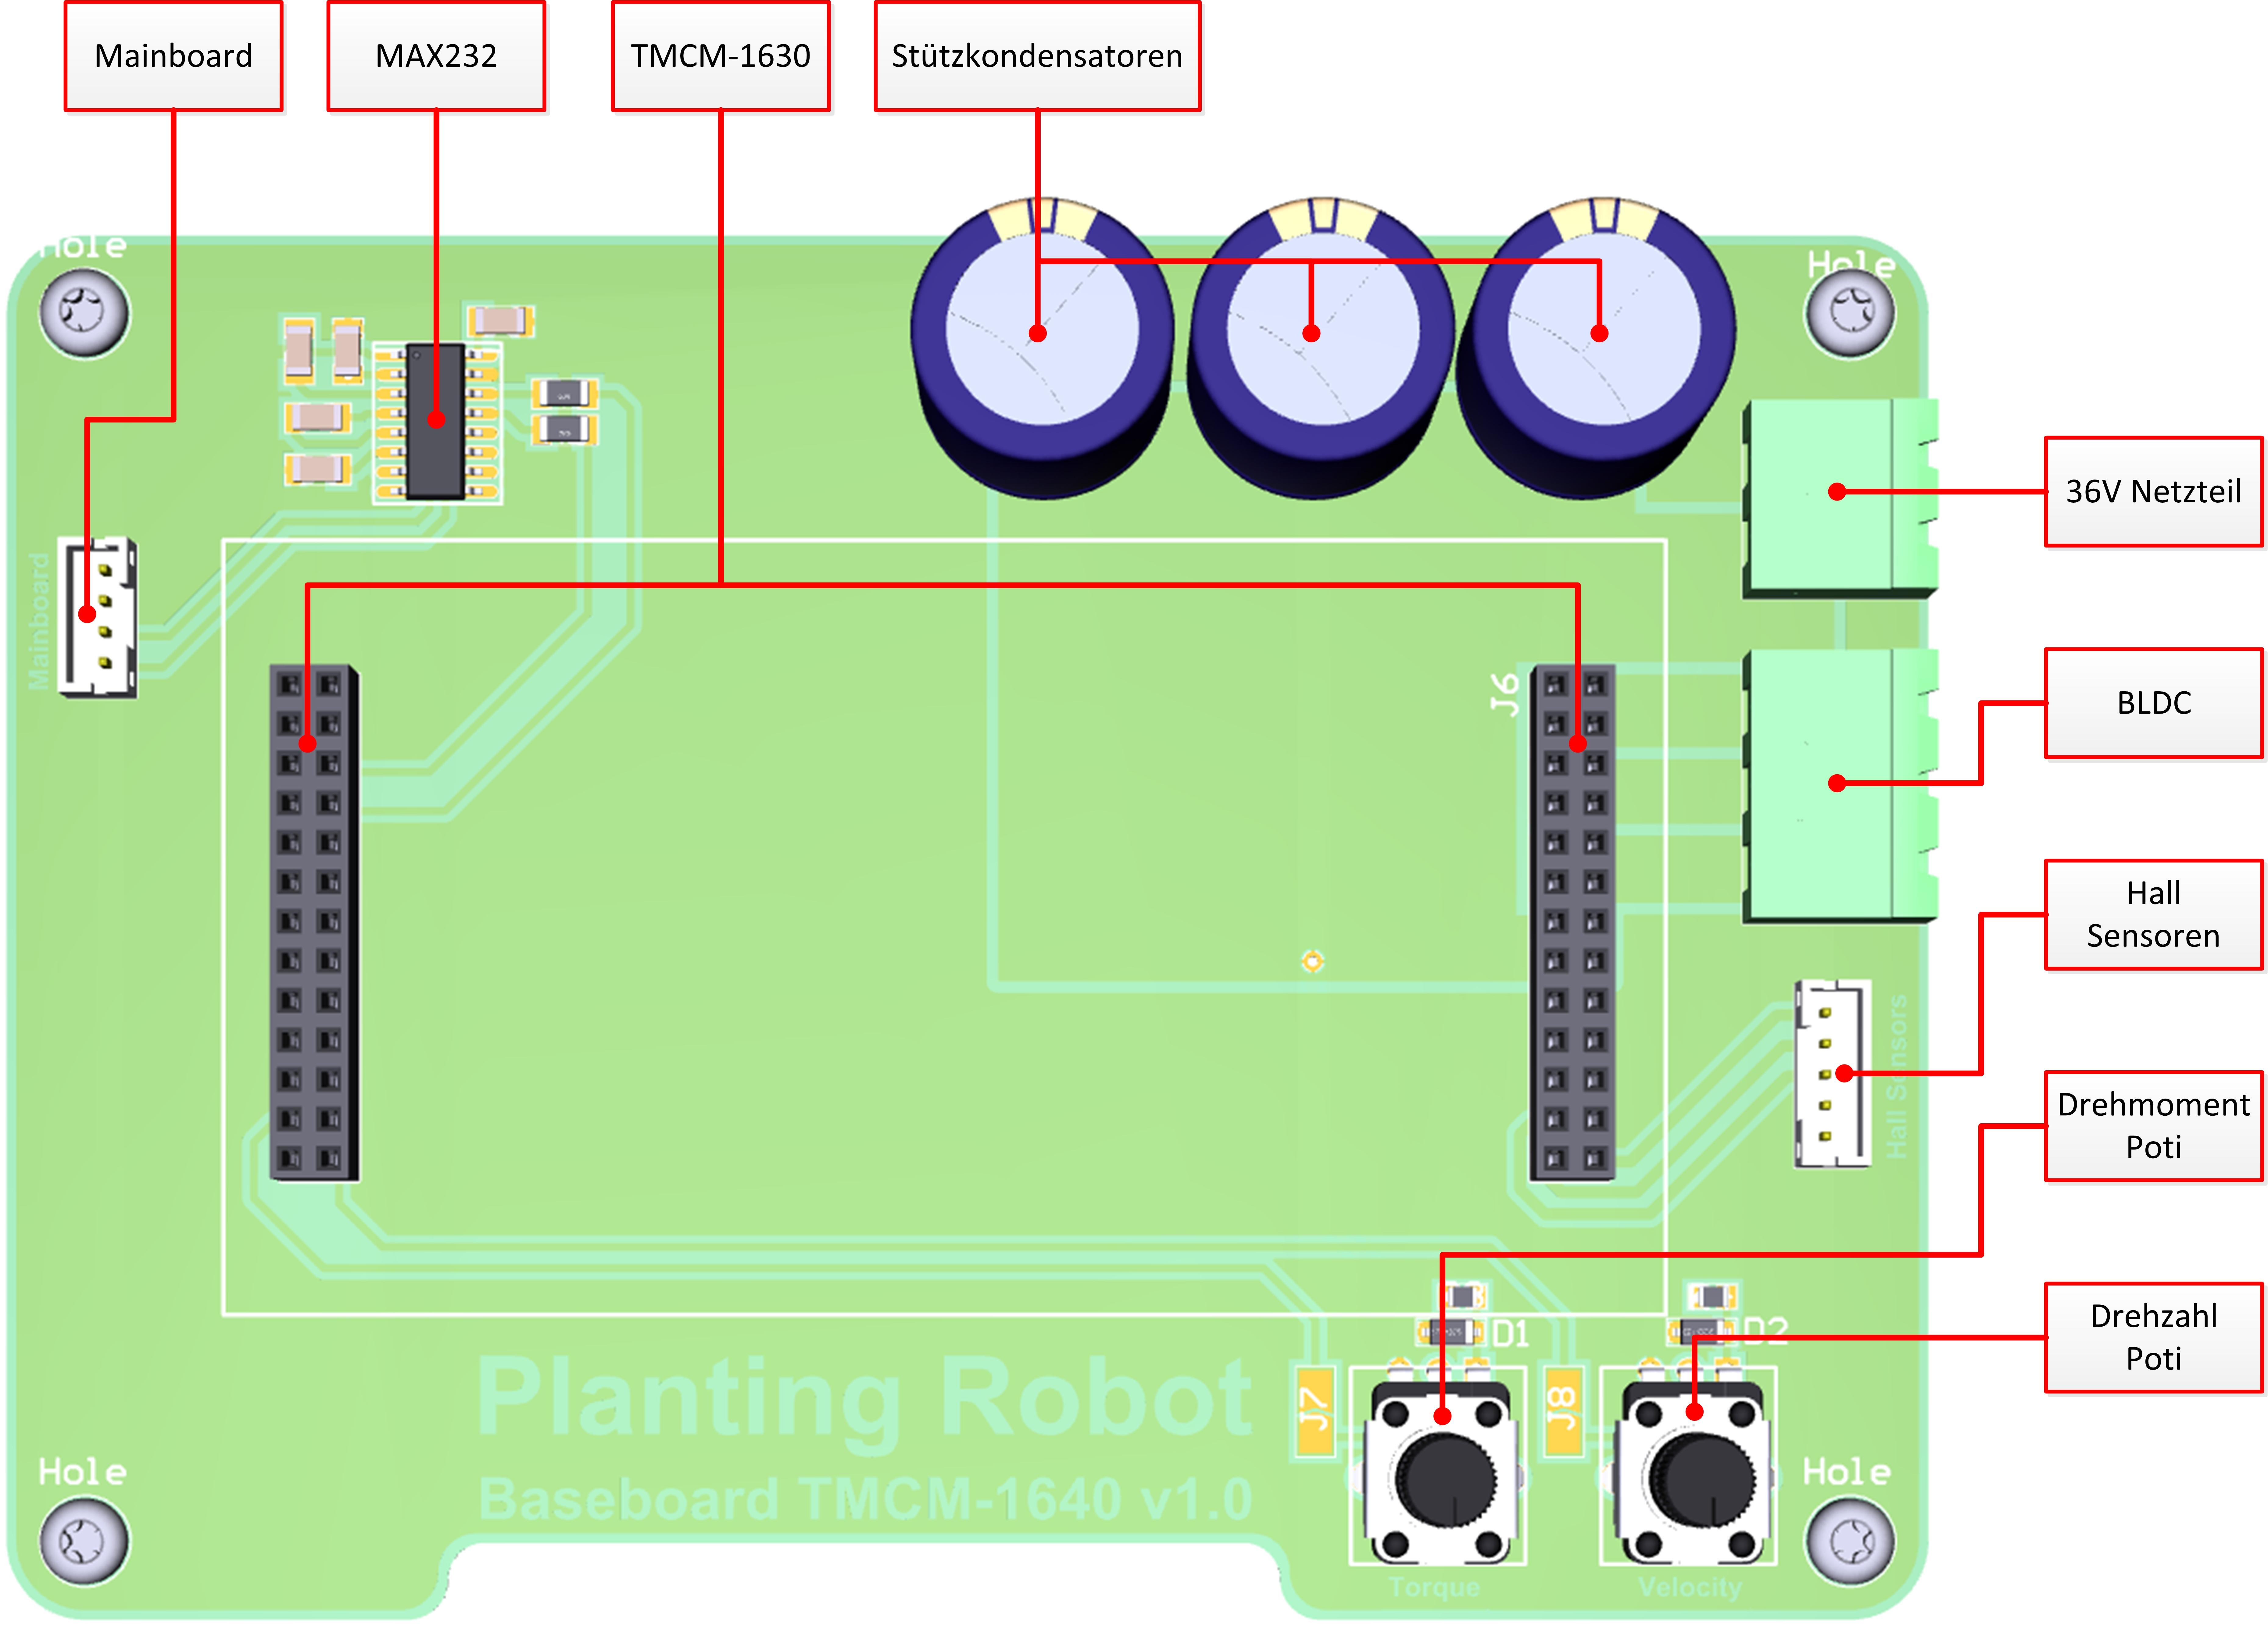
\includegraphics[width=1\textwidth]{Illustrationen/6-Umsetzung/Baseboard_3D_TOP.jpg}
	\caption{Baseboard PCB}
	\label{fig:Baseboard_3D}
\end{figure}

Die Verbindung zum Mainboard wir über einen 4 Poligen JST stecker realisiert. Auf ihn ist die UART Schnittstelle sowie das Signal Stop$\_$IN geführt. Das Stop $\_$IN Signal kann vom FRDM-Board auf GND gezogen werden um den Motorencontroller in den Not-Aus Modus zu bringen. Demnach wird der Motor gestoppt und der Controller muss durch ausschalten der Speisung zurückgesetzt werden. Der Schnittstellenwandler MAX232 von TI wandelt den UART TTL Pegel des FRDM-Board in den RS232 EIA Pegel des Motorencontrollers. Der Motorcontroller wird über zwei zweireihige Stiftleisten auf das Baseboard aufgesteckt. Dabei ist auf dem Motorencontroller TMCM-1630 \textbf{kein Verpolungsschutz} vorgesehen. Das Modul muss deshalb vor Inbetriebnahme zwingend wie folgt auf das Baseboard PCB gesteckt sein:

\begin{itemize}
	\item Der Bestückungsdruck des Motorcontrollers ist gleich ausgerichtet wie die Beschriftung $"$Planting Robot$"$ des Baseboard PCBs (nicht auf dem Kopf).
	\item Die LEDs des Motorcontrollers befinden sich auf der Seite des 4 Poligen JST Mainboard Steckers.
\end{itemize}

Um die Spannung auch bei hohen Laststromspitzen des BLDC Motors stabil zu halten werden drei 1mF Elektrolyt Kondensatoren Parallel zur Eingangsspannung geschaltet. Diese Vorgabe wurde dem Datenblatt des TMCM-1630 entnommen. Die 36V Eingangsspannung, sowie die Motorphasen werden über 90° Phoenix Stiftleisten der Serie MSTBA ausgeführt. Sie besitzen mit 10A den gleichen Nennstrom wie der Motorcontroller. Die Hall Sensoren des BLDC Motors werden über einen JST 5 Pol Stecker der Serie PH geführt. Für allfällige Testversuche während der Inbetriebnahme des BLDC Motors kann der Motorcontroller über die beiden Potentiometer im Standalone Modus betrieben werden. Die Analogsignale der beiden Potentiometer können über zwei lötbare Jumper vom Motorencontroller getrennt werden.